\section{D. Irga B. Naufal Fakhri}
\subsection{Buatlah library fungsi (file terpisah/library dengan nama NPM/textunderscore bar.py) untuk plot dengan jumlah subplot adalah NPM mod 3 + 2}

Ini adalah fungsi untuk membuat plot bar sesuai dengan hasil modulus:
\lstinputlisting[firstline=8, lastline=44]{src/6/1174066/Praktek/l1174066_bar.py}

Dan ini adalah cara memanggilnya:
\lstinputlisting[firstline=7, lastline=21]{src/6/1174066/Praktek/main.py}

\subsection{Buatlah library fungsi (file terpisah/library dengan nama NPM/textunderscore scatter.py) untuk plot dengan jumlah subplot adalah NPM mod 3 + 2}

Ini adalah fungsi untuk membuat plot scatter sesuai dengan hasil modulus:
\lstinputlisting[firstline=8, lastline=44]{src/6/1174066/Praktek/l1174066_scatter.py}

Dan ini adalah cara memanggilnya:
\lstinputlisting[firstline=23, lastline=37]{src/6/1174066/Praktek/main.py}

\subsection{Buatlah library fungsi (file terpisah/library dengan nama NPM/textunderscore pie.py) untuk plot dengan jumlah subplot adalah NPM mod 3 + 2}

Ini adalah fungsi untuk membuat plot pie sesuai dengan hasil modulus:
\lstinputlisting[firstline=8, lastline=50]{src/6/1174066/Praktek/l1174066_pie.py}

Dan ini adalah cara memanggilnya:
\lstinputlisting[firstline=39, lastline=53]{src/6/1174066/Praktek/main.py}

\subsection{Buatlah library fungsi (file terpisah/library dengan nama NPM/textunderscore pie.py) untuk plot dengan jumlah subplot adalah NPM mod 3 + 2}

Ini adalah fungsi untuk membuat subplot sesuai dengan hasil modulus:
\lstinputlisting[firstline=8, lastline=44]{src/6/1174066/Praktek/l1174066_plot.py}

Dan ini adalah cara memanggilnya:
\lstinputlisting[firstline=55, lastline=69]{src/6/1174066/Praktek/main.py}


\subsection{Keterampilan Penanganan Error}
\lstinputlisting[firstline=7, lastline=19]{src/6/1174066/Praktek/1174066_error.py}
%%%%%%%%%%%%%%%%%%%%%%%%%%%%%%%%%%%%%%%%%%%%%%%%%%%%%%%%%%%%%

\section{Chandra Kirana Poetra}
\subsection{Buatlah librari fungsi (file terpisah/library dengan nama NPM bar.py) untuk plot dengan jumlah subplot adalah NPM mod 3 + 2}

\lstinputlisting[firstline=8, lastline=28]{src/6/1174079/Praktek/1174079_Bar.py}

Cara memanggilnya:
\lstinputlisting[firstline=9, lastline=17]{src/6/1174079/Praktek/main.py}

\subsection{Buatlah librari fungsi (file terpisah/library dengan nama NPM scatter.py) untuk plot dengan jumlah subplot NPM mod 3 + 2}

\lstinputlisting[firstline=8, lastline=30]{src/6/1174079/Praktek/1174079_scatter.py}

Cara memanggilnya:
\lstinputlisting[firstline=9, lastline=17]{src/6/1174079/Praktek/main.py}

\subsection{Buatlah librari fungsi (file terpisah/library dengan nama NPM pie.py) untuk plot dengan jumlah subplot NPM mod 3 + 2}

\lstinputlisting[firstline=8, lastline=29]{src/6/1174079/Praktek/1174079_pie.py}

Cara memanggilnya:
\lstinputlisting[firstline=9, lastline=17]{src/6/1174079/Praktek/main.py}

\subsection{Buatlah librari fungsi (file terpisah/library dengan nama NPM plot.py) untuk plot dengan jumlah subplot NPM mod 3 + 2}

\lstinputlisting[firstline=8, lastline=30]{src/6/1174079/Praktek/1174079_plot.py}

Cara memanggilnya:
\lstinputlisting[firstline=9, lastline=17]{src/6/1174079/Praktek/main.py}


\subsection{Keterampilan Penanganan Error}
\lstinputlisting[firstline=8, lastline=25]{src/6/1174079/Praktek/error.py}

%%%%%%%%%%%%%%%%%%%%%%%%%%%%%%%%%%%%%%%%%%%%%%%%%%%%%%%%%%%%%%%%%%%%%%%%%%%%%%%%%%%%%%%%%%%%%%%%%%%%%%%%%%%%%%%%%%%%%%%%%%

\section{Fanny Shafira Damayanti | 1174069}
\subsection{Keterampilan Pemrograman}
\begin{enumerate}
\item Jawaban NO 1
\lstinputlisting[firstline=8, lastline=30]{src/6/1174069/Praktek/1174069_bar.py}

\begin{figure}[H]
	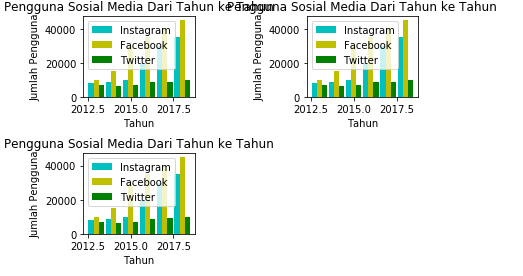
\includegraphics[width=12cm]{figures/6/1174069/Praktek/bar.png}
	\centering
	\caption{Hasil compile membuat fungsi Bar Plot .}
\end{figure}

\item Jawaban NO 2
\lstinputlisting[firstline=8, lastline=30]{src/6/1174069/Praktek/1174069_scatter.py}

\begin{figure}[H]
	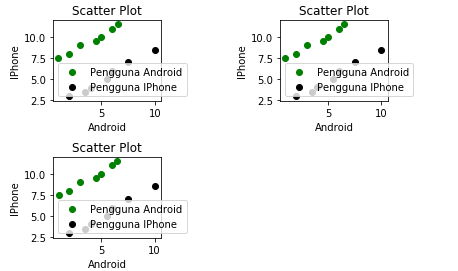
\includegraphics[width=12cm]{figures/6/1174069/Praktek/scatter.png}
	\centering
	\caption{Hasil compile membuat fungsi Scatter Plot .}
\end{figure}

\item Jawaban NO 3
\lstinputlisting[firstline=8, lastline=31]{src/6/1174069/Praktek/1174069_pie.py}

\begin{figure}[H]
	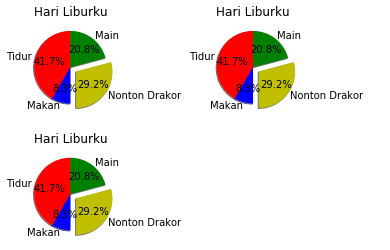
\includegraphics[width=12cm]{figures/6/1174069/Praktek/pie.png}
	\centering
	\caption{Hasil compile membuat fungsi Pie Plot .}
\end{figure}

\item Jawaban NO 4
\lstinputlisting[firstline=8, lastline=35]{src/6/1174069/Praktek/1174069_plot.py}

\begin{figure}[H]
	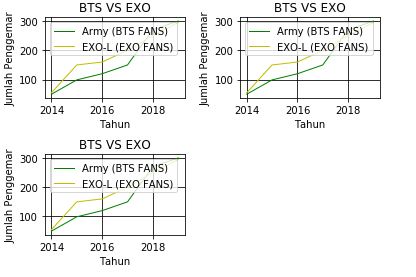
\includegraphics[width=12cm]{figures/6/1174069/Praktek/plot.png}
	\centering
	\caption{Hasil compile membuat fungsi Plot .}
\end{figure}

\end{enumerate}

\subsection{Penanganan Error}
Tuliskan  peringatan  error  yang  didapat  dari  mengerjakan  praktek  keenam  ini, dan  jelaskan  cara  penanganan  error  tersebut. dan  Buatlah  satu  fungsi  yang menggunakan try except untuk menanggulangi error tersebut.

\hfill \break
Peringatan error di praktek kelima ini, yaitu:
\begin{itemize}
	\item Syntax Errors
	Syntax Errors adalah suatu keadaan saat kode python mengalami kesalahan penulisan. Solusinya adalah memperbaiki penulisan kode yang salah.
	
	\item Name Error
	NameError adalah exception yang terjadi saat kode melakukan eksekusi terhadap local name atau global name yang tidak terdefinisi. Solusinya adalah memastikan variabel atau function yang dipanggil ada atau tidak salah ketik.
	
	\item Type Error
	TypeError adalah exception yang akan terjadi apabila pada saat dilakukannya eksekusi terhadap suatu operasi atau fungsi dengan type object yang tidak sesuai. Solusi dari error ini adalah mengkoversi varibelnya sesuai dengan tipe data yang akan digunakan.
\end{itemize}

\lstinputlisting[caption = Kode program membuat fungsi penanganan error., firstline=160, lastline=177]{src/6/1174069/Praktek/1174069.py}

\subsection{Screenshoot Plagiat}
\begin{figure}[H]
	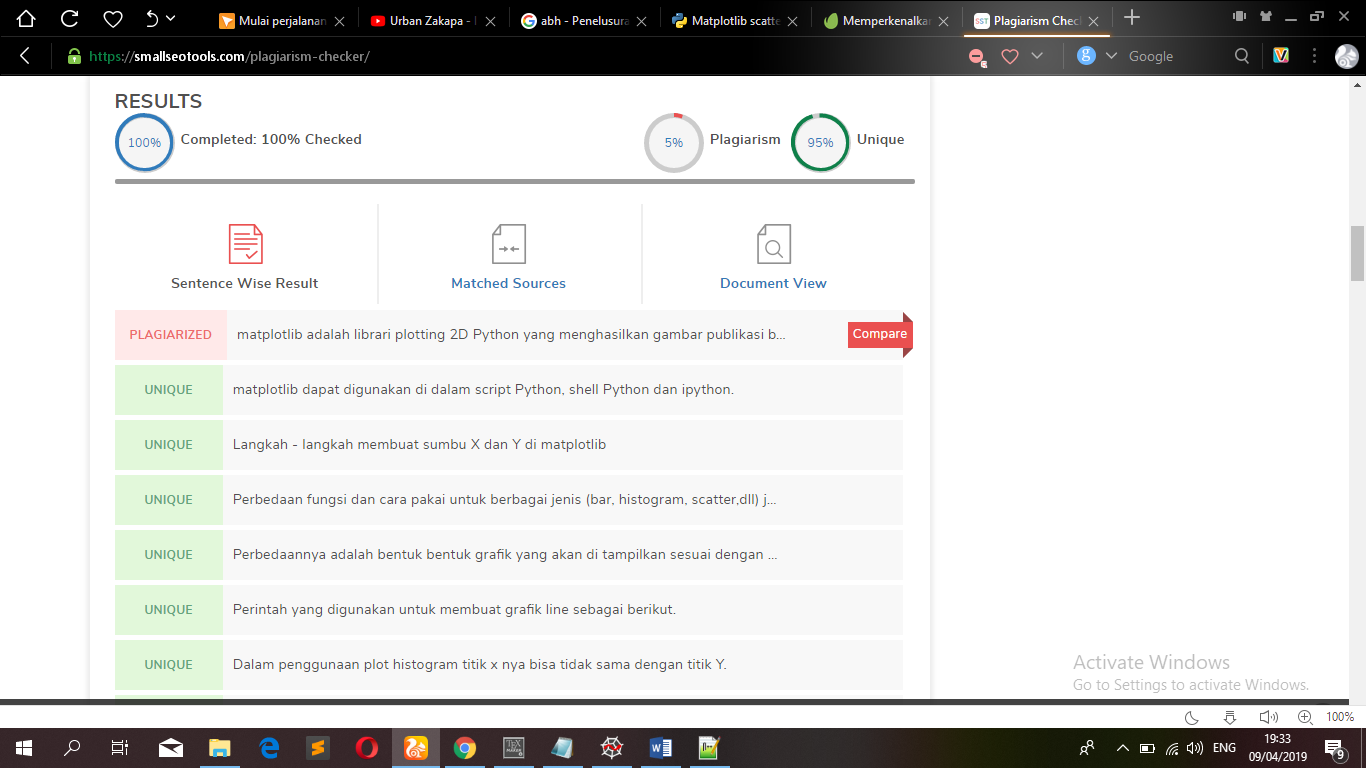
\includegraphics[width=12cm]{figures/6/1174069/Praktek/plagiat.png}
	\centering
\end{figure}

